\chapter{Sensor tests}

%\section{Digital}
%    \subsection{Interface tests}
%    \subsection{Software tests}

\section{Power}
    \subsection{LDO stabilisation}
        Voltage after LDO was measured against time, to calculate the delay between power enablement and measurement start. The time-domain graph is shown in figure \ref{LDO_rise_time}. Delay was estimated to be around \SI{1}{\second}.

        \begin{figure}[H]
            \centering
            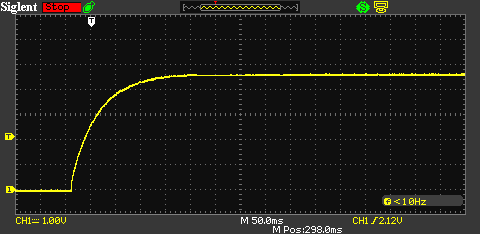
\includegraphics[width=0.8\paperwidth]{img/07/rise_time.png}
            \caption{LDO rise time}
            \label{LDO_rise_time}
        \end{figure}

    \subsection{Power consumption}
        The current drawn during readout is about \SI{25}{\milli\ampere} at \SI{5}{\volt} rail, so the power consumption of the sensor equals \SI{0.125}{\watt}.

\section{Current source}
    Current source was tested on HP 34970A - 6 1/2 digit multimeter, with 200 power line cycle integration enabled.

    \subsection{Noise}
        The noise of the current source was measured for a long period of time, taking a sufficient number of samples. The results (\ref{Current_Stability}) show that the noise floor is below specification for this meter.

        \begin{figure}[H]
            \centering
            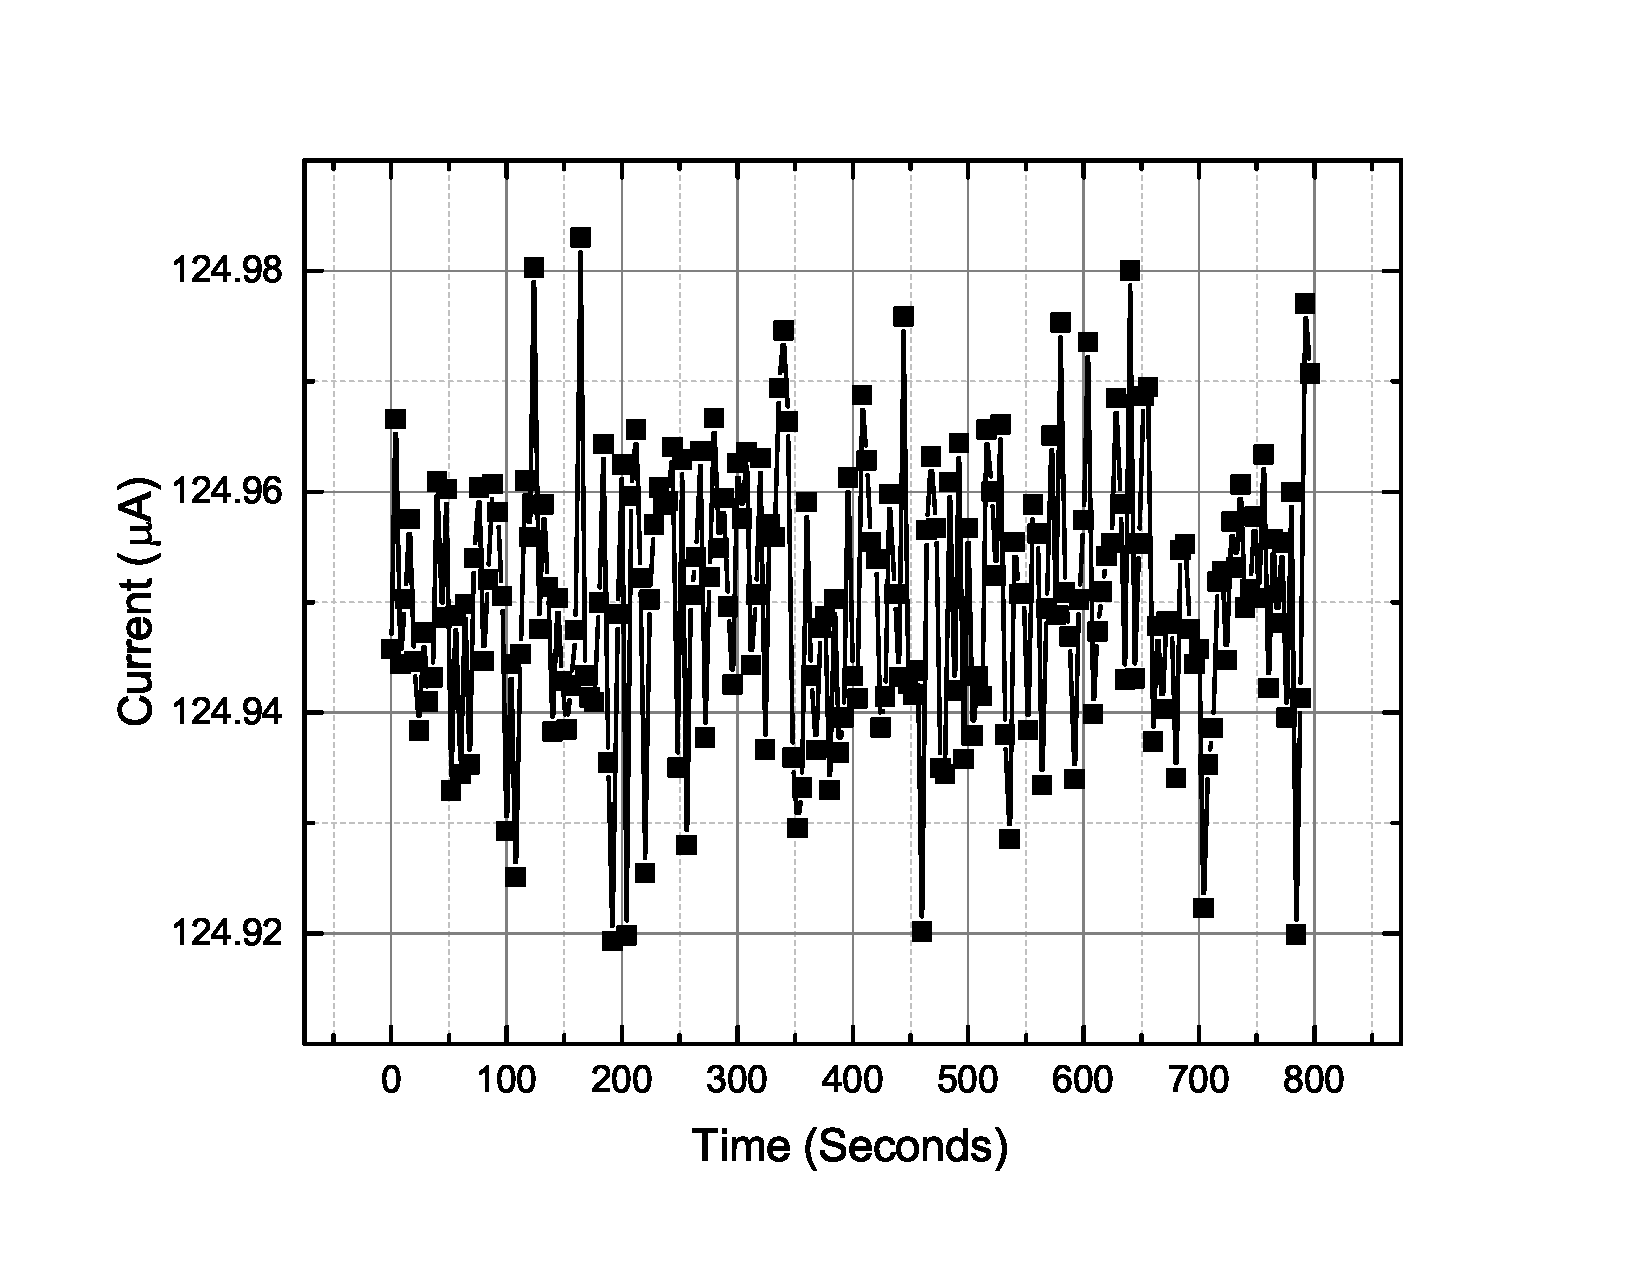
\includegraphics[width=0.6\paperwidth]{img/07/current_time.eps}
            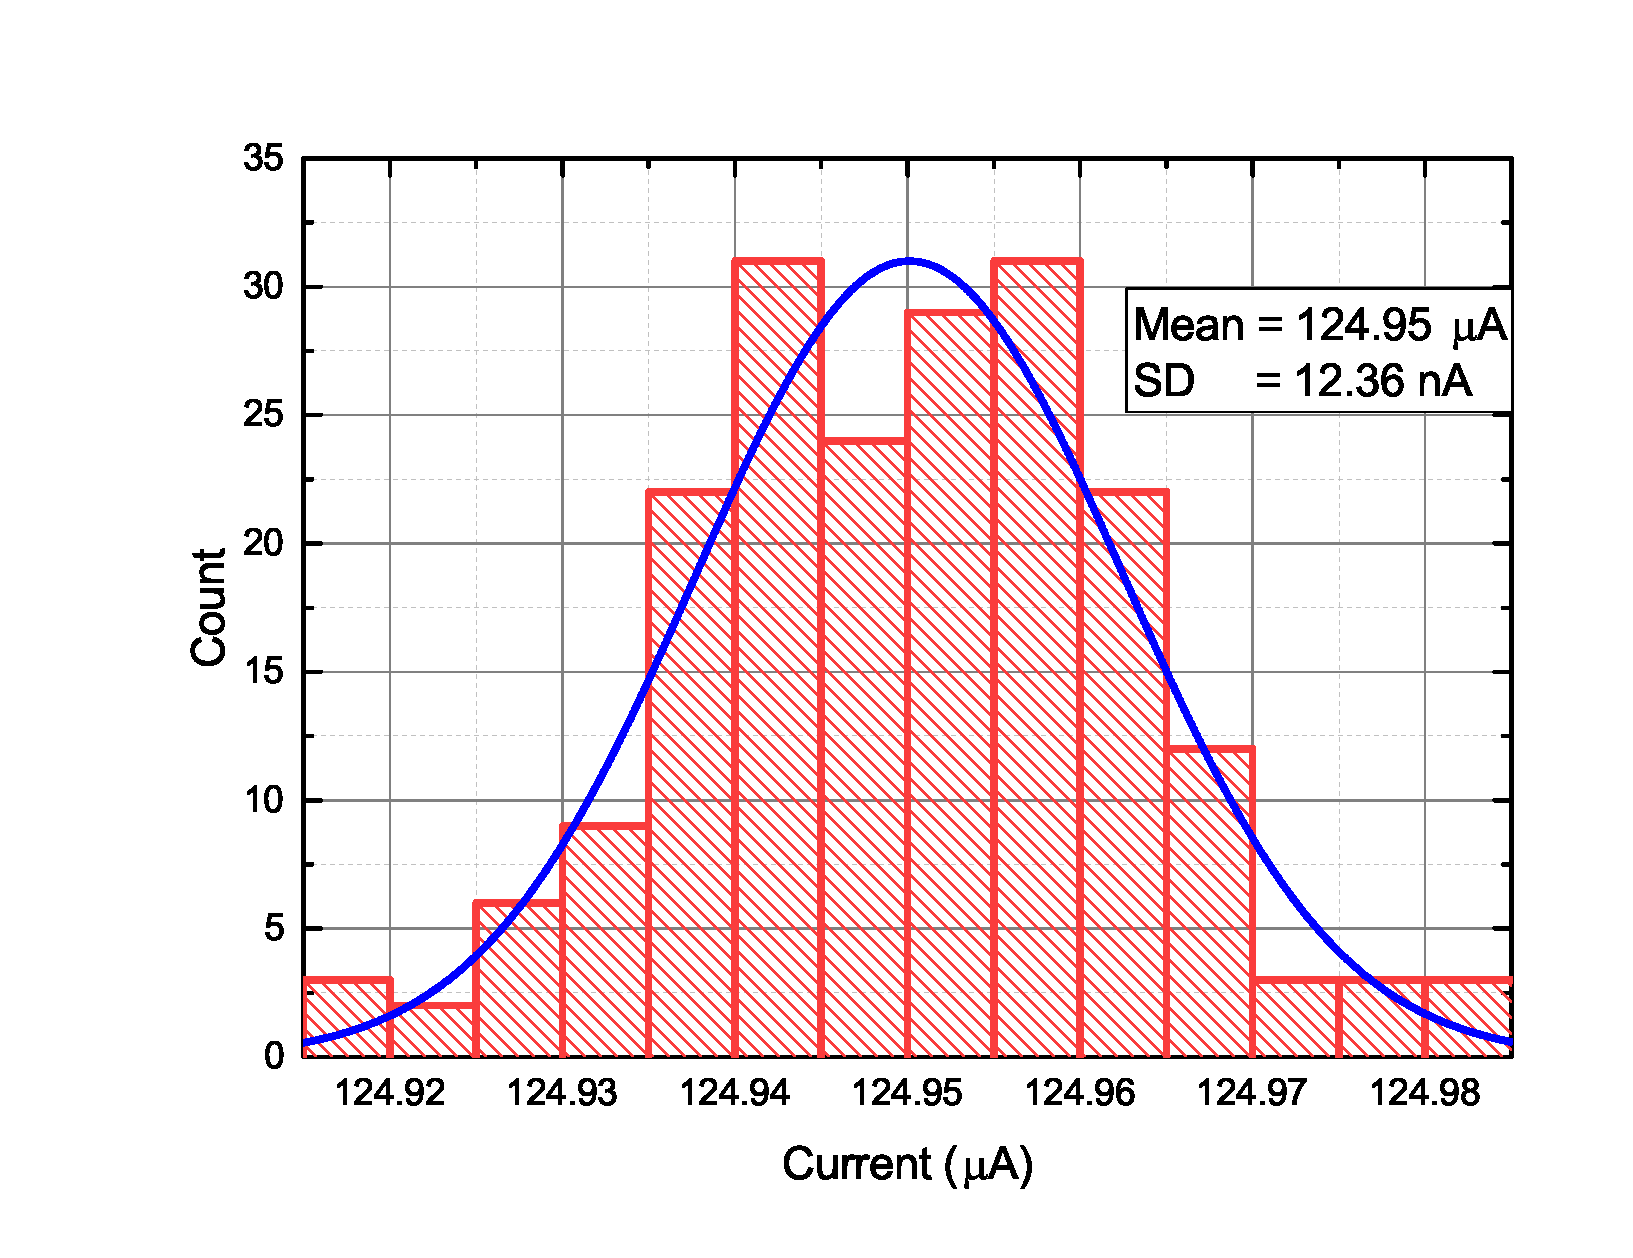
\includegraphics[width=0.6\paperwidth]{img/07/current_hist.eps}
            \caption{LDO rise time}
            \label{Current_Stability}
        \end{figure}

    \subsection{Load range}
        Output load was changed identically as it was in simulation, to test its fidelity. Simulation and build models show the same range and stability - confirming the design. The current source works as intended for loads between \SI{1.4}{\kilo\ohm} and \SI{22.5}{\kilo\ohm} (figure \ref{Current_sensor_output_characteristics}).
        \begin{figure}[H]
            \centering
            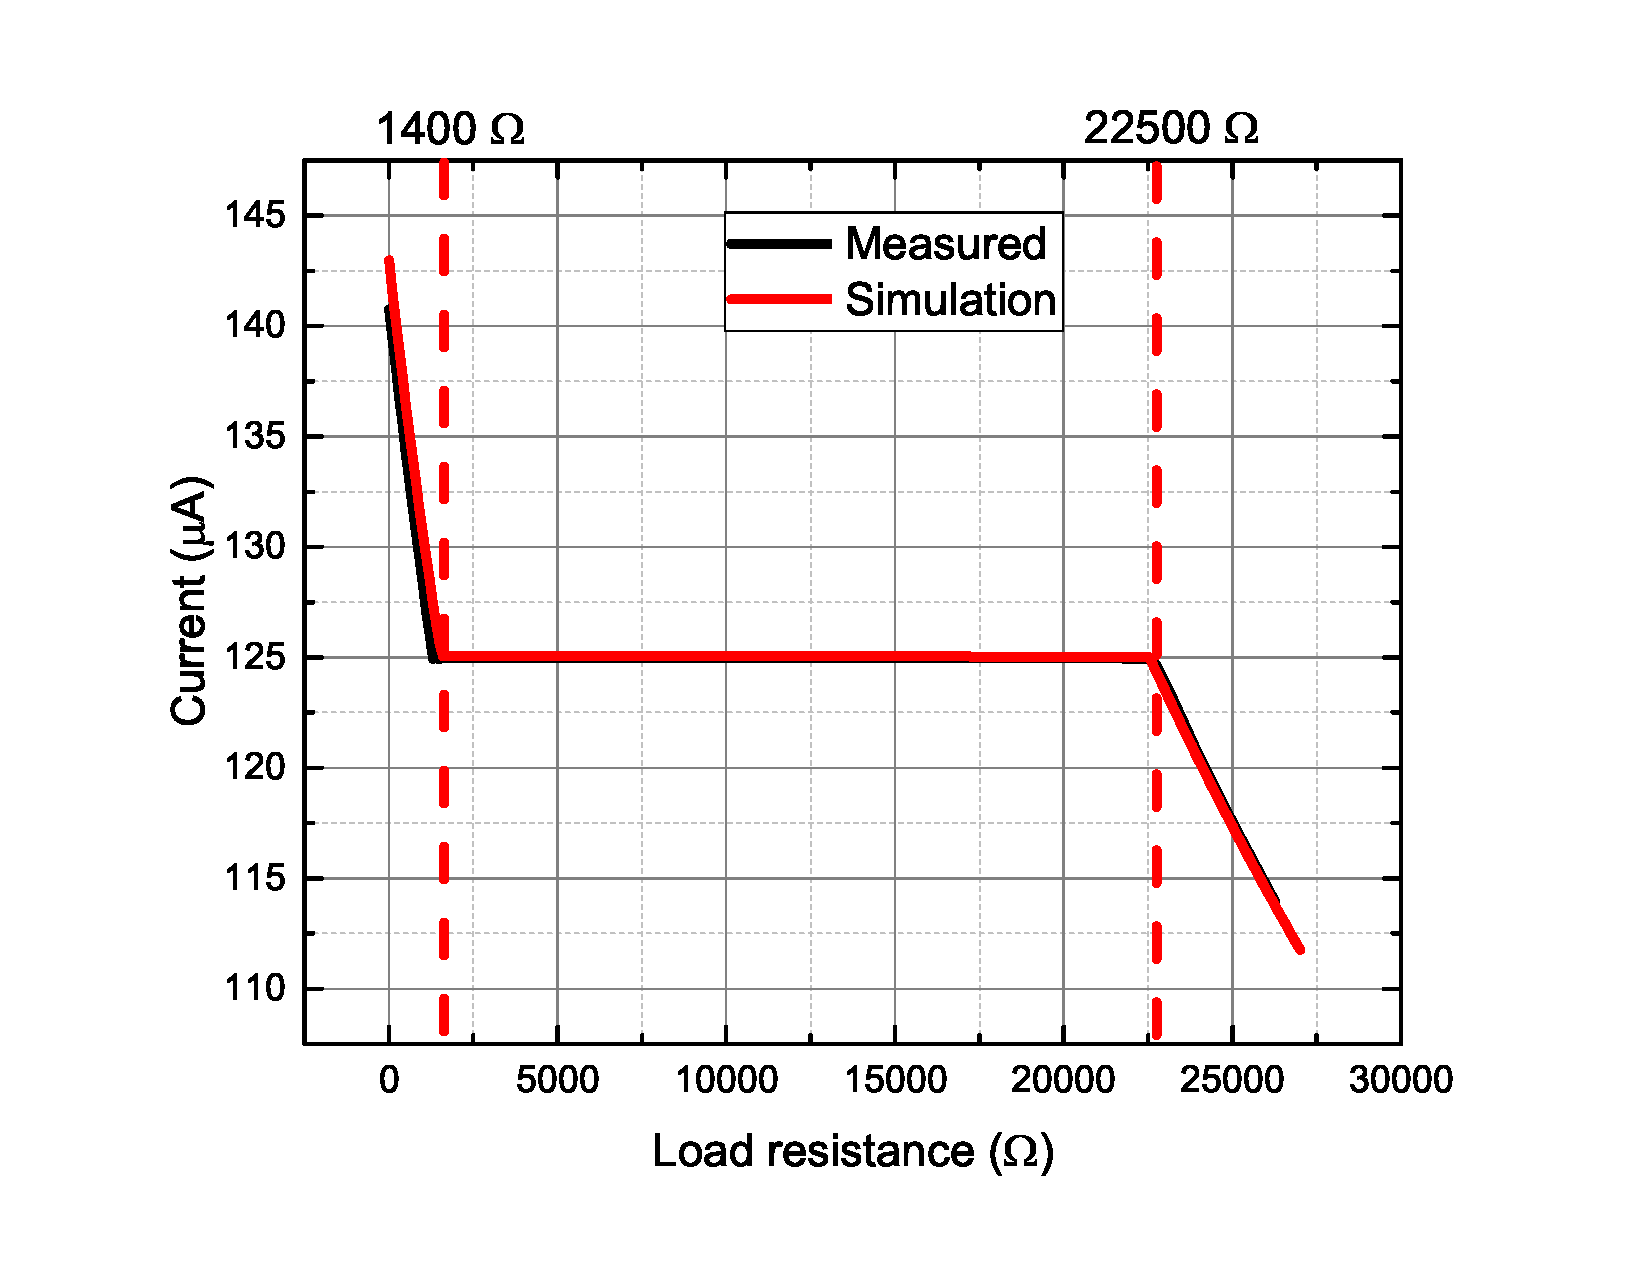
\includegraphics[width=0.9\paperwidth]{img/07/output_resistance.eps}
            \caption{Current sensor output characteristics}
            \label{Current_sensor_output_characteristics}
        \end{figure}

    \subsection{Temperature stability}
        Temperature was swept from $20$ to \SI{70}{\degreeCelsius}, no detectable changes were measured by the available meter, therefore it is assumed that current source fluctuates lower than about \SI{20}{\nano\ampere} in this temperature range.

\section{MOS settling}
    After enabling the measurement channel for the threshold voltage it takes a lot of time to fully stabilize its value. Instead of pre-enabling, same time method was used. ADC takes measurement of threshold voltage at precisely specified time after enabling power. In figure \ref{MOS_settling} 10 runs of measured voltage vs time are plotted, proving this method is stable within \SI{20}{\uV}.

    \begin{figure}[H]
        \centering
        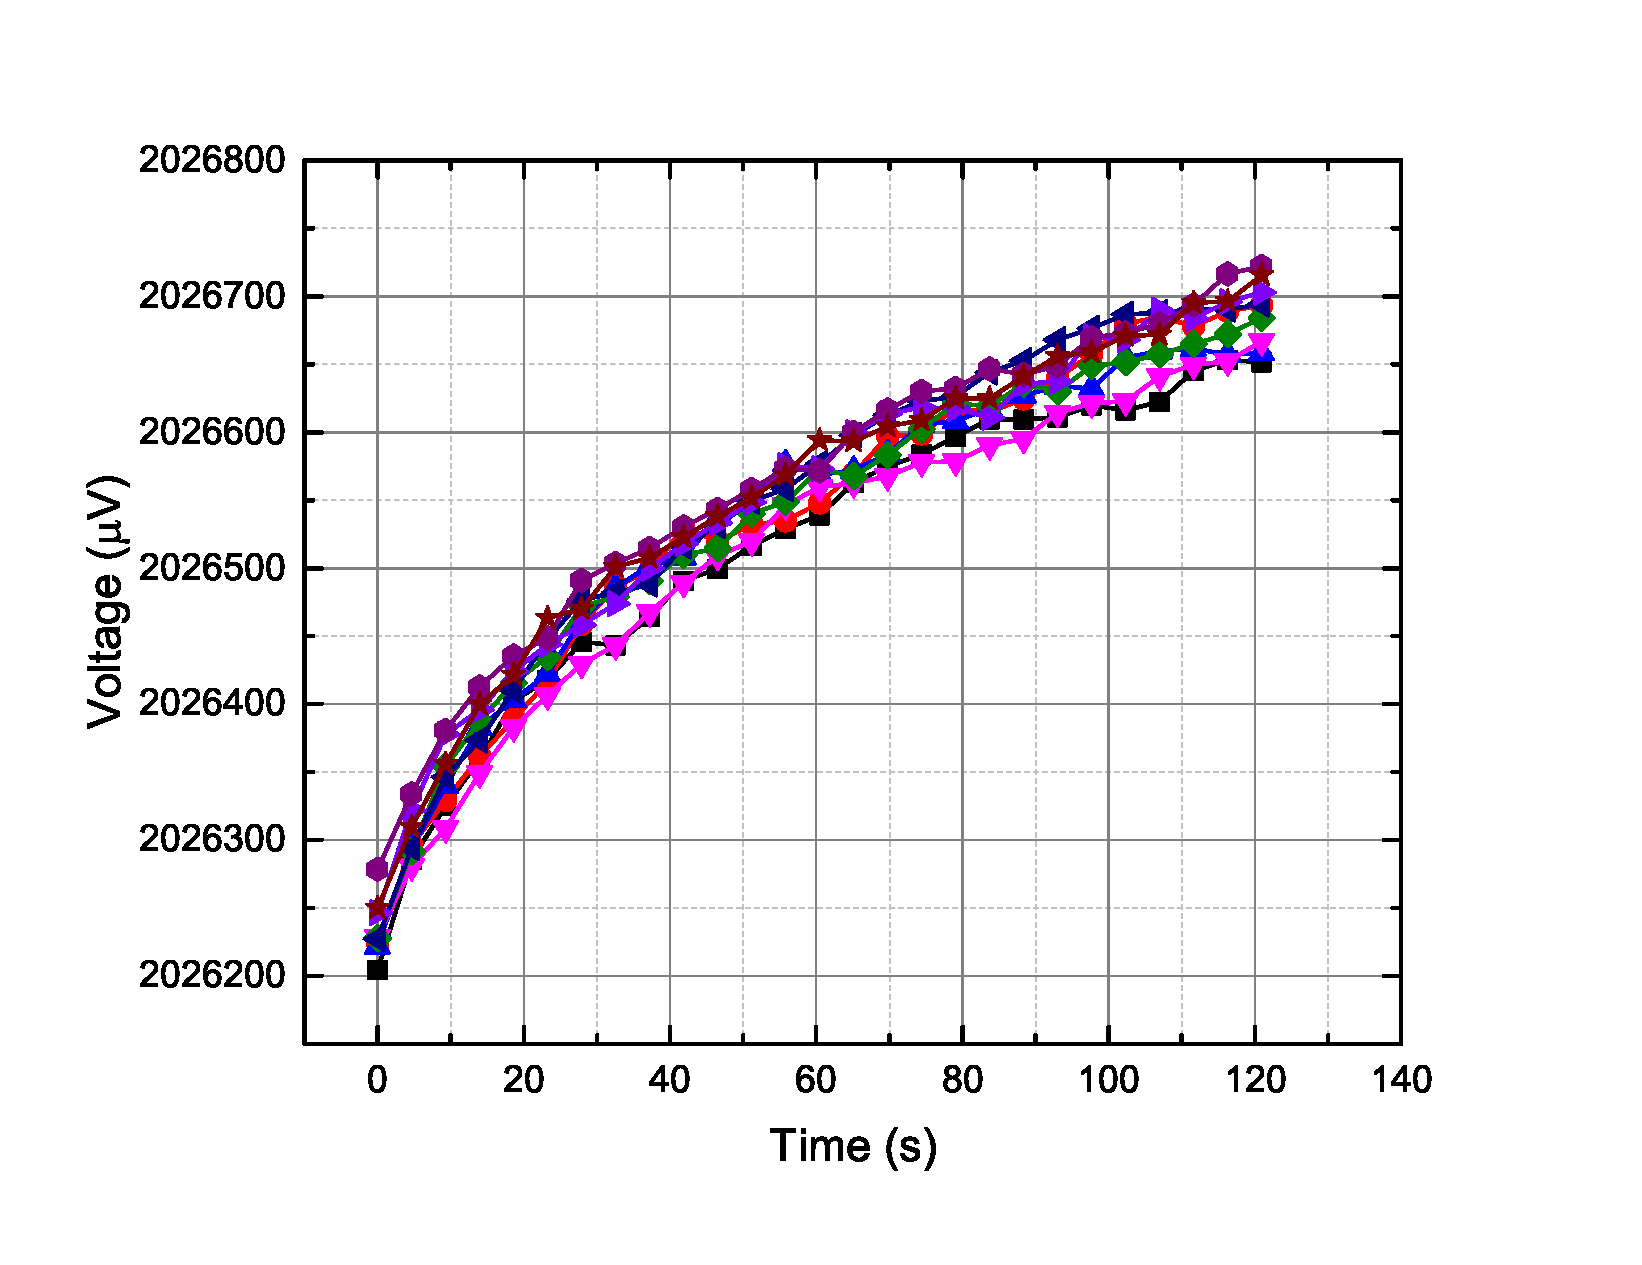
\includegraphics[width=0.8\paperwidth]{img/07/MOS_settling.eps}
        \caption{10 runs of MOS voltage setting}
        \label{MOS_settling}
    \end{figure}

\section{Measurement noise}
    The most important noise figure is system noise - ADC reading noise floor during nominal work.

    Because even the smallest temperature changes cause the ADC reading to shift (due to threshold/diode voltage shift) this efect had to be eliminated to measure noise. For this purpose a DC notch filter was used in post-processing, to eliminate any DC bias during measurement. The sampling frequency of the ADC was its nominal rate of \SI{0.25}{\hertz}. An example of filtration is shown in figure \ref{notch_DC_example}.

    \begin{figure}[H]
        \centering
        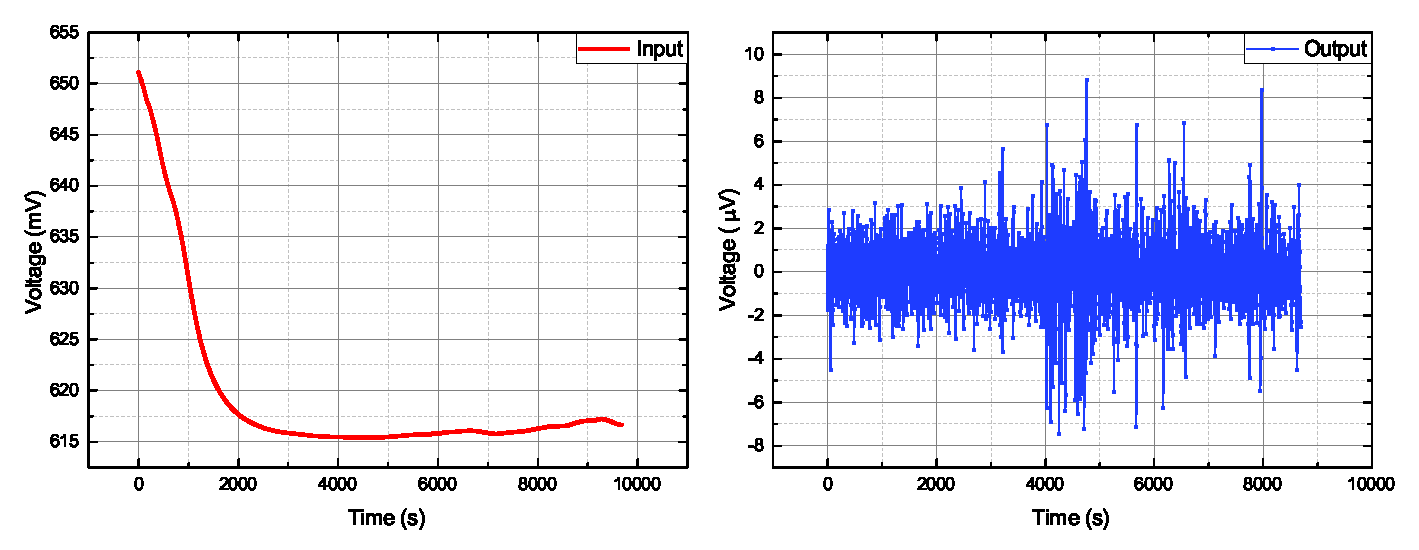
\includegraphics[width=0.8\paperwidth]{img/07/filterBeforeAfter.eps}
        \caption{Input and output of DC notch filter}
        \label{notch_DC_example}
    \end{figure}

    \subsection{Diode}
        \begin{figure}[H]
            \centering
            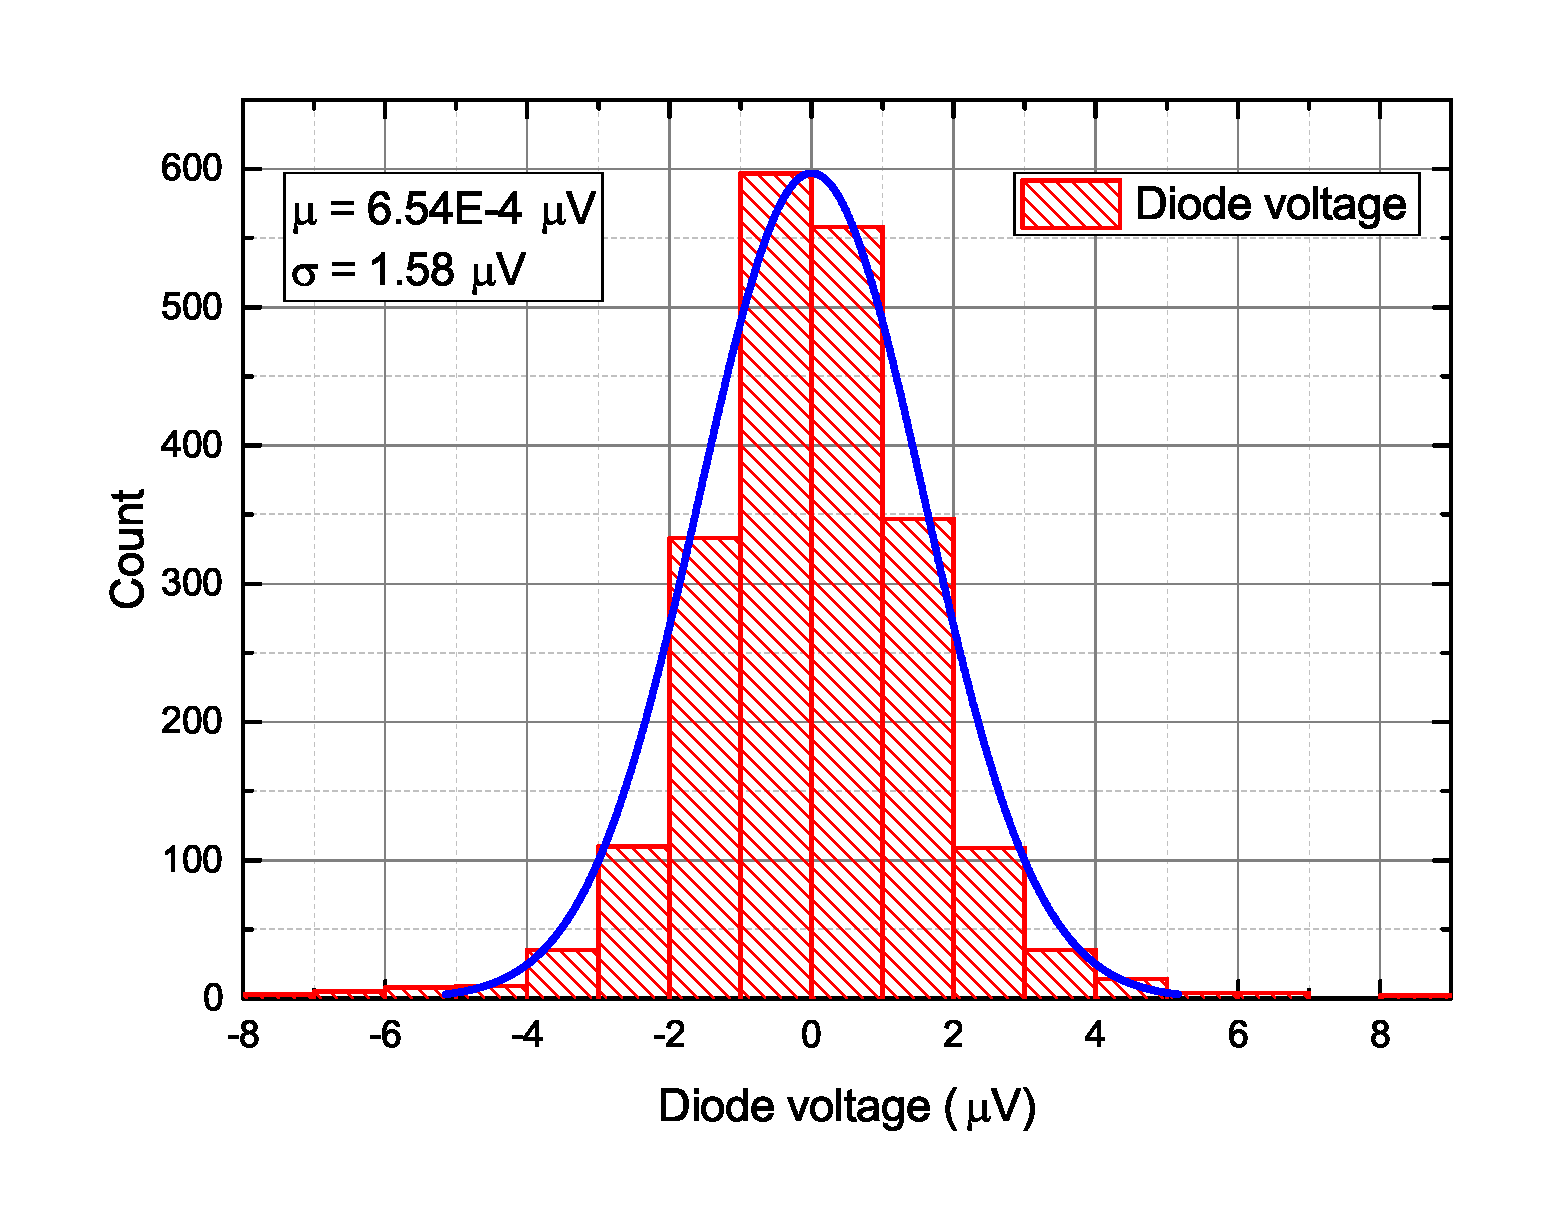
\includegraphics[width=0.6\paperwidth]{img/07/diodeVoltage.eps}
            \caption{Measured noise on body temperature channel}
        \end{figure}

        Noise on the temperature measurement channel has a standard deviation of $\SI{1.58}{\uV}$
    \subsection{Threshold voltage}
        \begin{figure}[H]
            \centering
            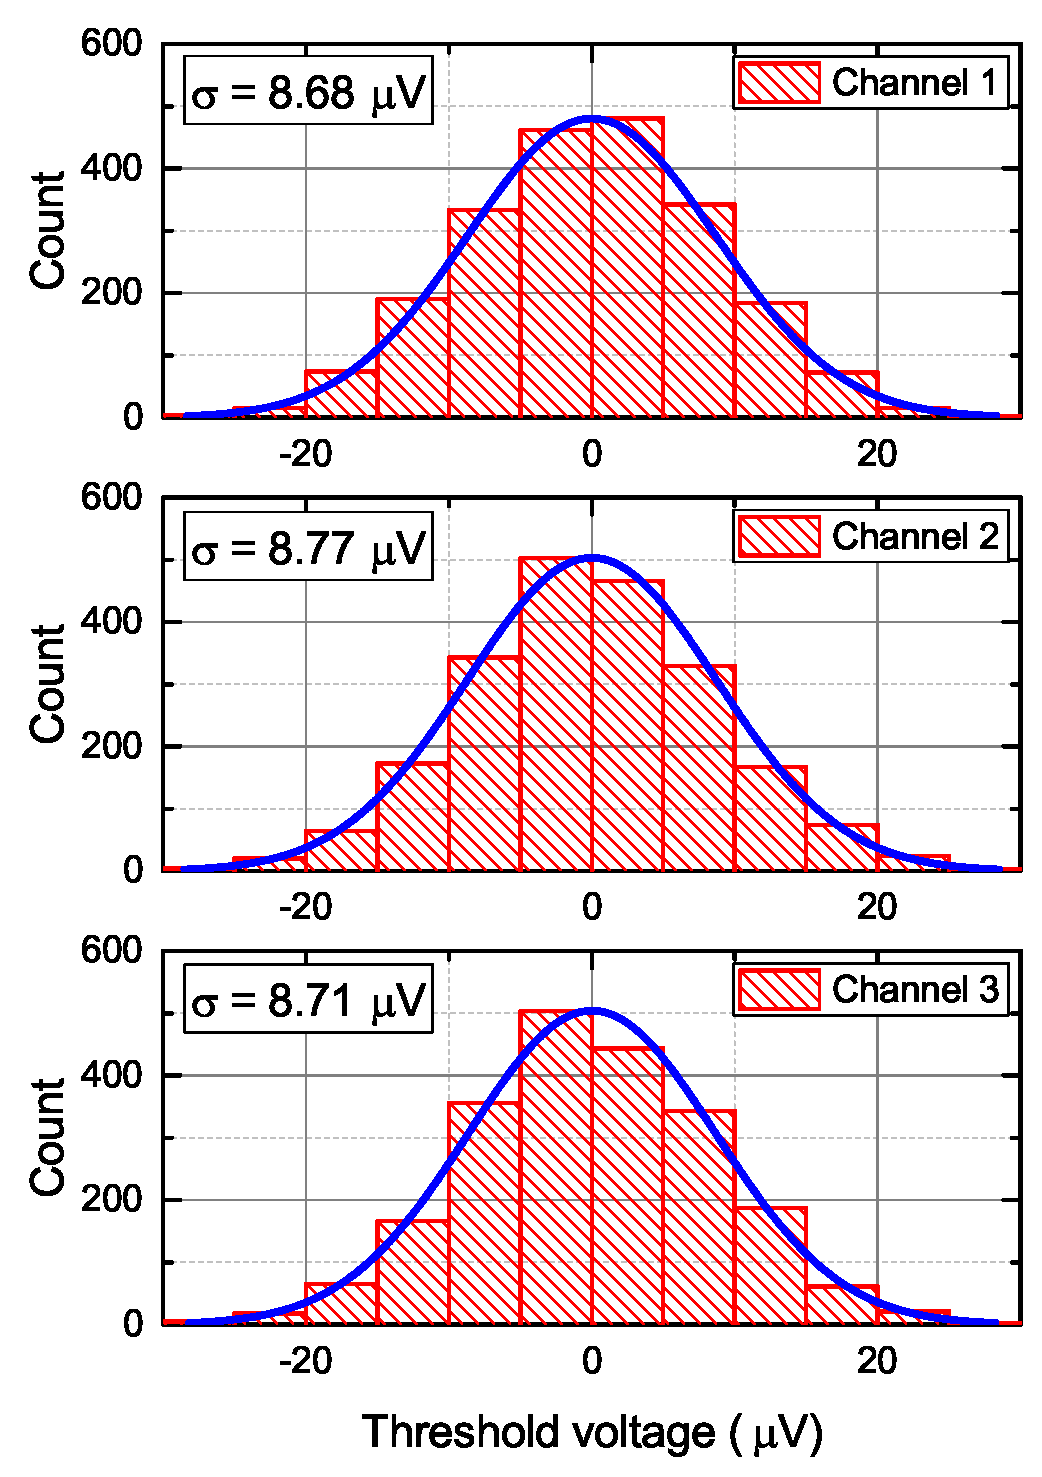
\includegraphics[width=0.6\paperwidth]{img/07/thresholdVoltageHistograms.eps}
            \caption{Measured noise on body temperature channel}
        \end{figure}

        Noise on the threshold voltage measurement channel has standard deviations of \SI{8.68}{\uV}, \SI{8.77}{\uV}, \SI{8.71}{\uV}.



    \subsection{Interpretation}
        Because the only difference between the temperature and threshold voltage channels is the semiconductor itself, the noise source can be estimated from the significant difference between them.

        The dependence between threshold voltage and drain current for this type of transistor was measured by M. Gumiela:
        $$I_D~[\mu A] = 410.376 \cdot (V_{TH} - 1.56457)^2 \text{~~~~~~Source: \ref{CD4007_p-MOSFET_transfer}}$$
        $$\frac{\textit{d}}{\textit{d}V_{TH}} I_D= 820.75 \cdot (-1.56 + V_{TH}) = \SI{439.46}{\uA/V} \text{~~~@ operating point}$$
        $$\textit{d}I_d = \SI{3.82}{\nA}$$
        Estimated equivalent current source have RMS value of $I_{N~RMS} = \SI{3.82}{\nA}$.

        This value is the same order of magnitude as calculated: reference voltage LT1634 has low-frequency noise of $U_N = \SI{15}{\uV}$ [TODO], this value is sensed directly across a series resistor, therefore $I_{NOISE} = U_N/R = \SI{1.5}{\nA}$. The left-hand side part of the noise equation can originate from different parts of the circuit, thermal and shot noise etc. % Noise output from LTSpice:



\section{Temperature characteristics}
    By placing the sensor in a thermal chamber and sweeping the temperature from \SI{0}{\degreeCelsius} up to \SI{75}{\degreeCelsius} temperature dependency charts were obtained for the device.

    \subsection{Diode}
        The diode response (figure \ref{Body_diode_temperature_dependency}) is almost ideally linear.
        \begin{figure}[H]
            \centering
            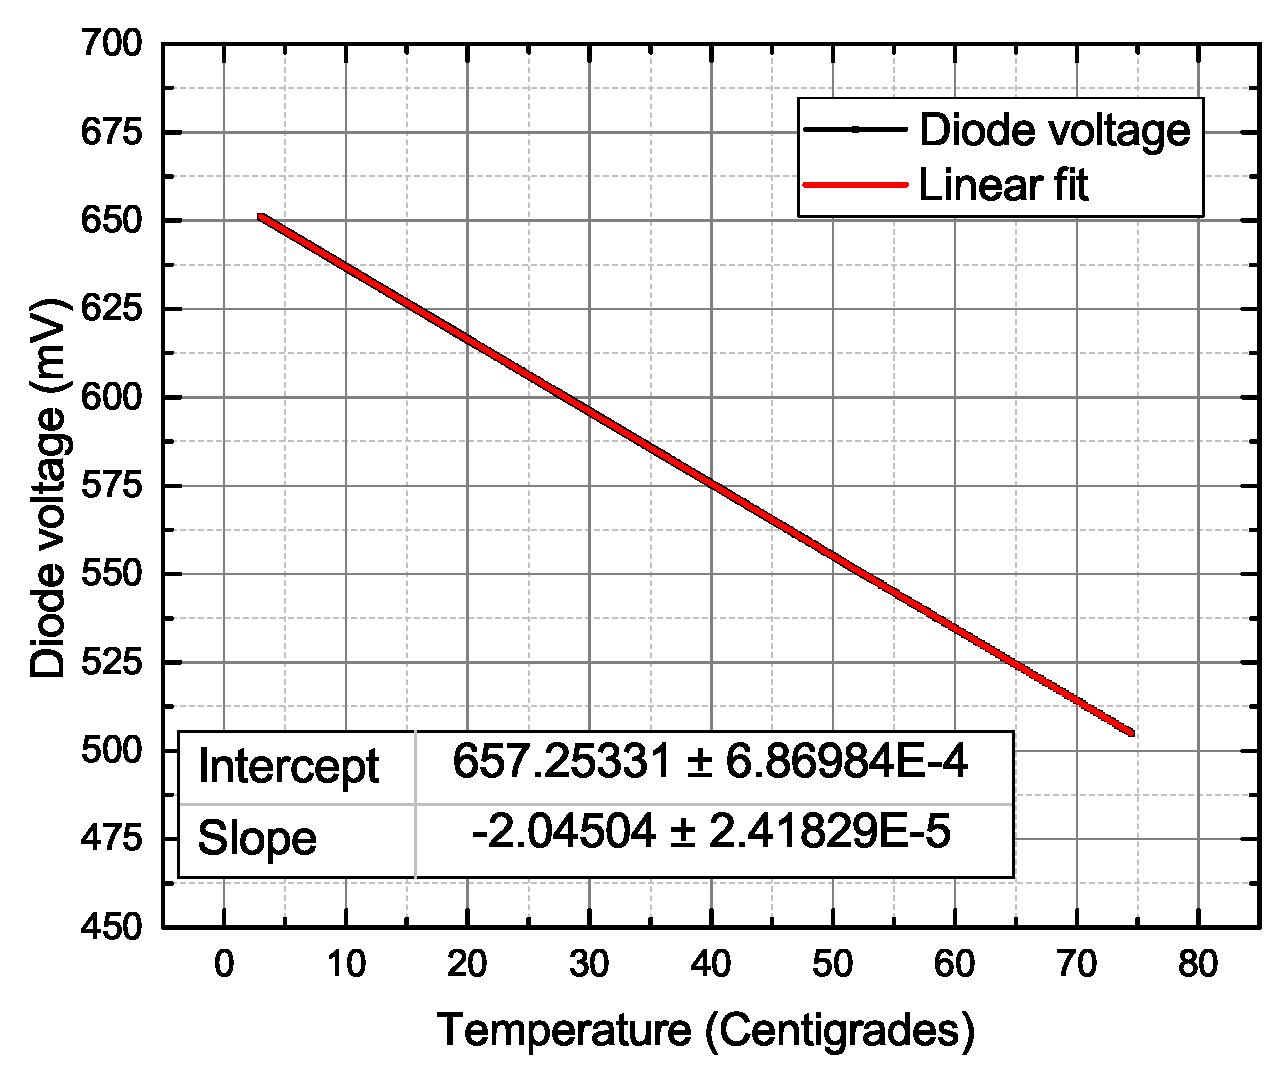
\includegraphics[width=0.6\paperwidth]{img/07/diodeVsTemperature.eps}
            \caption{Body diode temperature dependency}
            \label{Body_diode_temperature_dependency}
        \end{figure}


    \subsection{Threshold voltage}
        The threshold voltage (figure \ref{threshold_voltage_temperature_dependency}) tends to be non-linear, but it can be approximated as a quadratic function. Equation used: $V_{TH} = a \cdot t^2 + b \cdot t + c$, fitted parameters are shown in table \ref{vth_fit_params}.
        \begin{figure}[H]
            \centering
            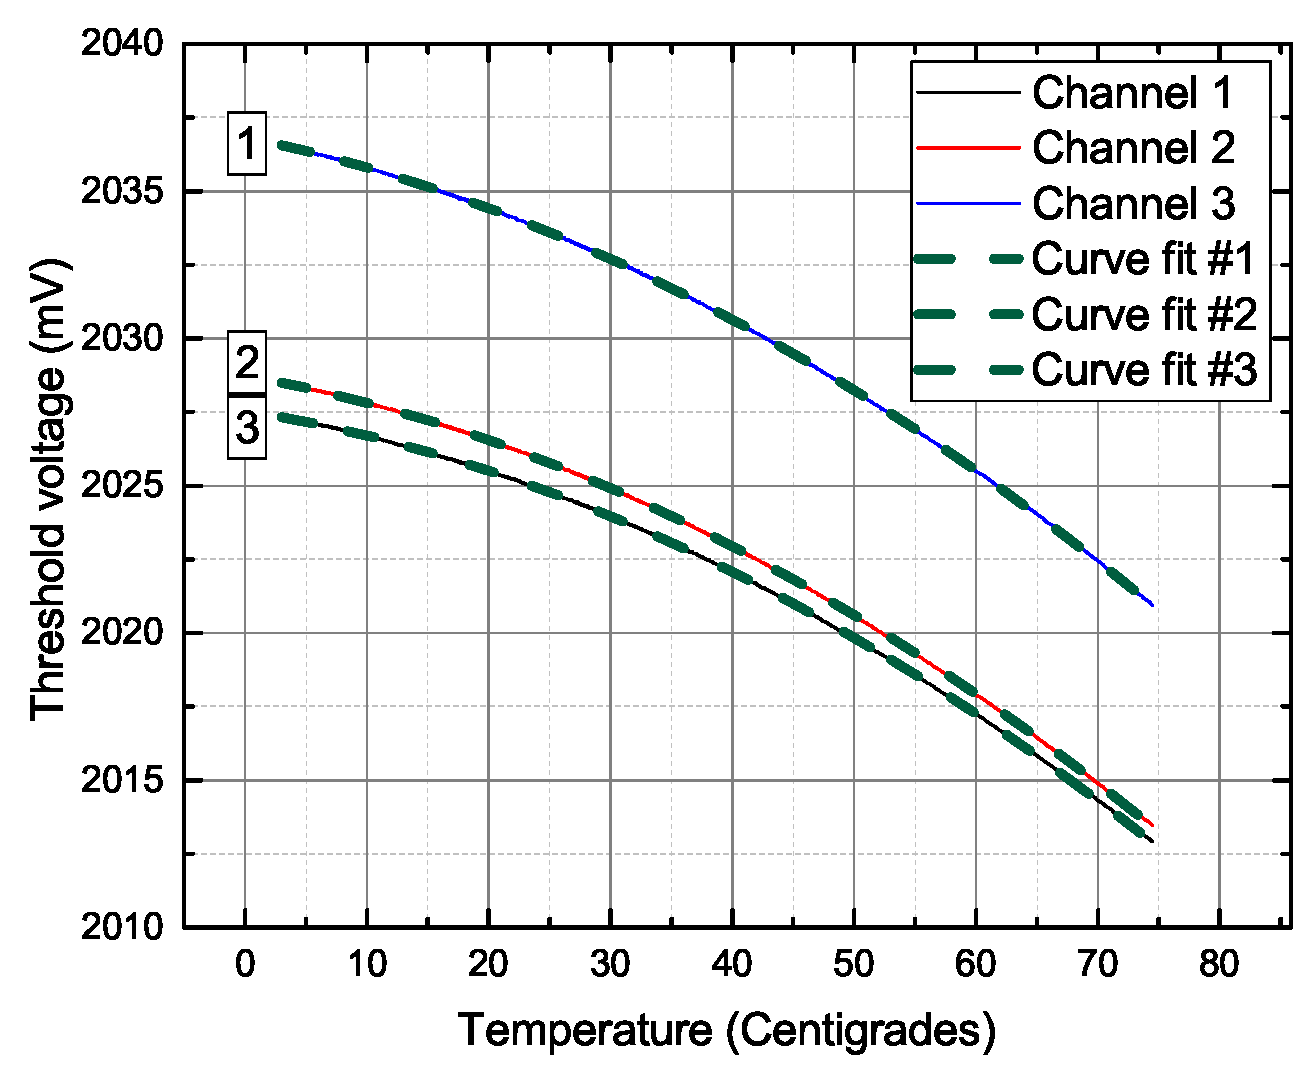
\includegraphics[width=0.6\paperwidth]{img/07/thresholdVoltageTemperatureDependency.eps}
            \caption{Threshold voltage temperature dependency}
            \label{threshold_voltage_temperature_dependency}
        \end{figure}

        \begin{table}[H]
            \begin{center}
                \begin{tabular}{c|c|c|c}
                    Channel & a & b & c \\ \hline
                    ch 1 & $-0.00174~\pm~1.17011e-6$ & $-0.06692~\pm~8.33551e-5$ & $2027.53424~\pm~0.00125$ \\
                    ch 2 & $-0.00176~\pm~1.07318e-6$ & $-0.07437~\pm~7.64496e-5$ & $2028.72804~\pm~0.00114$ \\
                    ch 3 & $-0.00169~\pm~1.12071e-6$ & $-0.08736~\pm~7.98355e-5$ & $2036.83689~\pm~0.00119$ \\
                \end{tabular}
            \end{center}
            \caption{Temperature compensation results}
            \label{vth_fit_params}
        \end{table}

\section{Temperature compensation stability}
    The sensor should be compensated for temperature, with the assumption that temperature characteristic curves will not change during irradiation.

    During temperature sweep, data was gathered and post-processed, applying thermal compensation (given by charts \ref{Body_diode_temperature_dependency} and \ref{threshold_voltage_temperature_dependency}). In full sensing range, the sensor output shifts off the maximum $\SI{104}{\uV}$, which reflects TID measurement accuracy of about \SI{\pm 1}{\rad}. Note that TID dependency was not tested, but assumed according to \cite{COTSMosfetsGarcia}. Detailed accuracies are listed in table \ref{Temperature_compensation_results}.


    \begin{figure}[H]
        \centering
        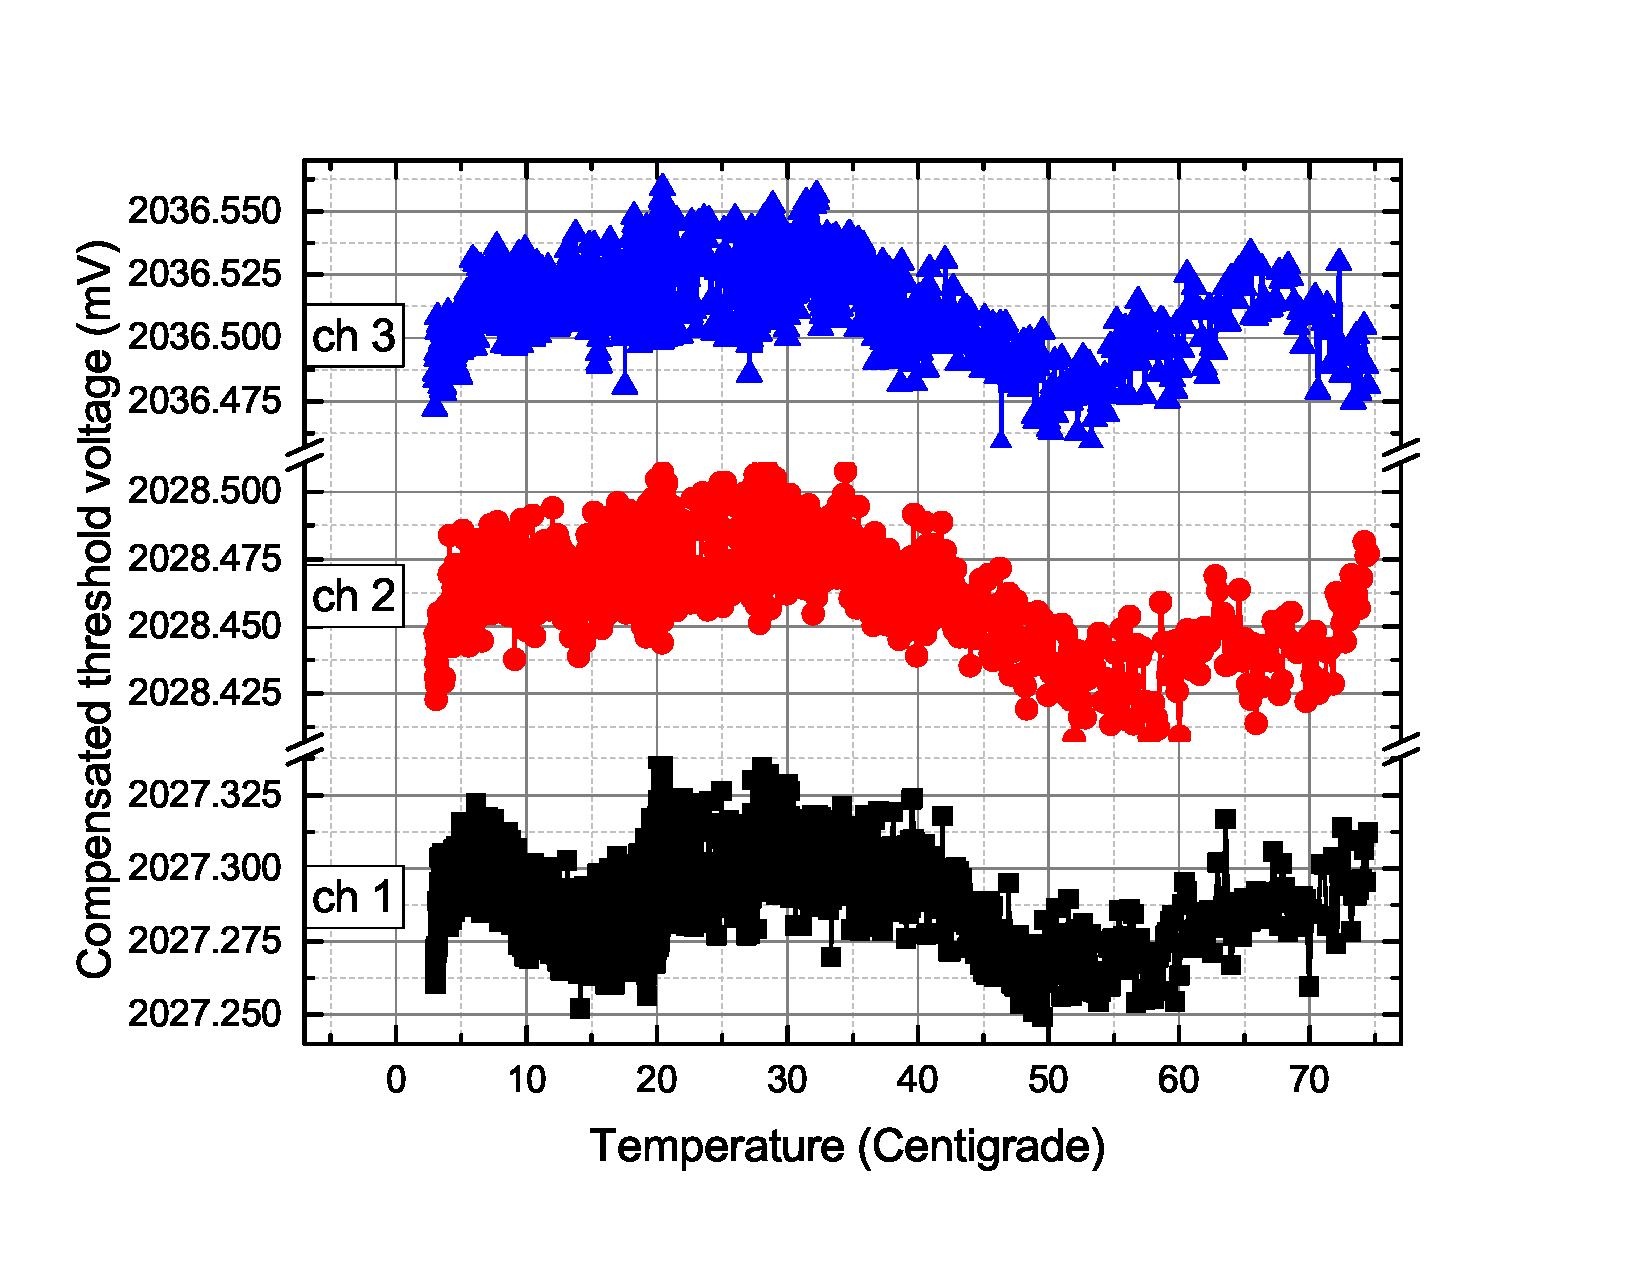
\includegraphics[width=0.8\paperwidth]{img/07/compensatedThresholdVoltage.eps}
        \caption{Threshold voltage temperature compensation}
        \label{threshold_voltage_temperature_compensation}
    \end{figure}

    \begin{table}[H]
        \begin{center}
            \begin{tabular}{c|c|c|c}
                Channel & Standard deviation & Maximum difference & Accuracy ($3~\sigma$) \\ \hline
                ch 1 & \SI{15.13}{\uV} & \SI{89.40}{\uV} & \SI{\pm~0.0108}{\gray} = \SI{\pm~1.08}{\rad} \\
                ch 2 & \SI{16.27}{\uV} & \SI{103.24}{\uV} & \SI{\pm~0.0109}{\gray} = \SI{\pm~1.09}{\rad} \\
                ch 3 & \SI{15.36}{\uV} & \SI{101.26}{\uV} & \SI{\pm~0.0103}{\gray} = \SI{\pm~1.03}{\rad} \\
            \end{tabular}
        \end{center}
        \caption{Temperature compensation results}
        \label{Temperature_compensation_results}
    \end{table}
